\setchapterpreamble[u]{\margintoc}
\chapter{Third Lecture}
\labch{lec3}

% Will contain only signal flow graphs, system stability & singularities are shifted to lec 4 ... 

\section{Signal Flow Graphs}
\labsec{sec3.1}

\begin{figure}[h]
	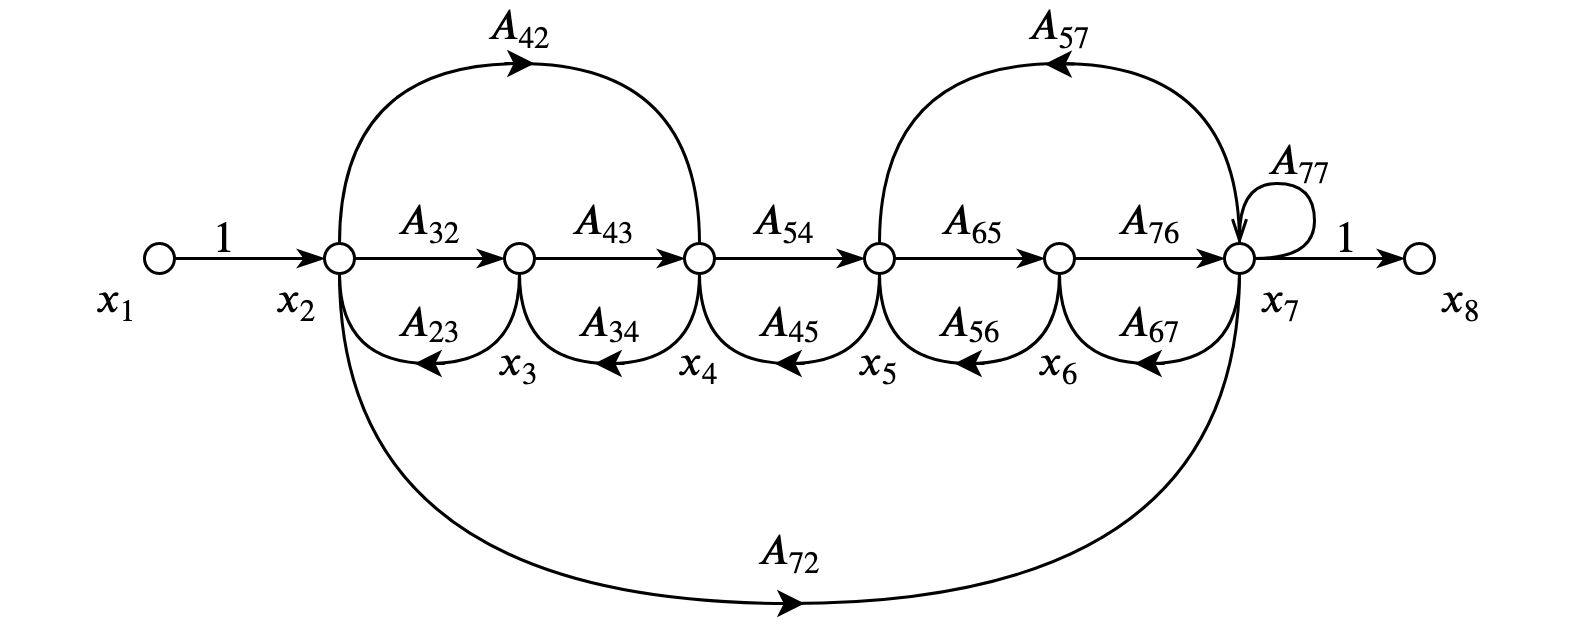
\includegraphics{lec3/Signal Flow}
	\caption{Signal flow general graph.}
\end{figure}

\subsection[Nodes]{Nodes\linkT{Reference: Feedback control system analysis and synthesis}}

\begin{description}
	\item[Source Nodes]  Represent independent variables and have only outgoing branches. ($x_1$)
	\item[Sink Nodes]  Represent dependent variables and have only incoming branches. ($x_8$)
	\item[Mixed Nodes]  Have both incoming and outgoing branches. ($x_2 \to x_7$)
\end{description}

\subsection[Paths]{Paths\linkS{http://imtiazhussainkalwar.weebly.com/feedback-control-systems-modeling-and-analysis.html}}

% [+0.42cm] is needed to allign with graphs that is not in margin, so -0.42 is good to allign with text.
% 0.4233401538135892 cm = 12 pt

\begin{description}
	\item[Forward Path]  From the input node to the output node.
		\begin{marginfigure}[-0.4233401538135892cm]
			\includegraphics{lec3/Forwards}
		\end{marginfigure}
	\vspace{2.7 cm}
	
	\item[Feedback loop]  Originates and terminates on the same node.
		\begin{marginfigure}[+0.4233401538135892cm]
			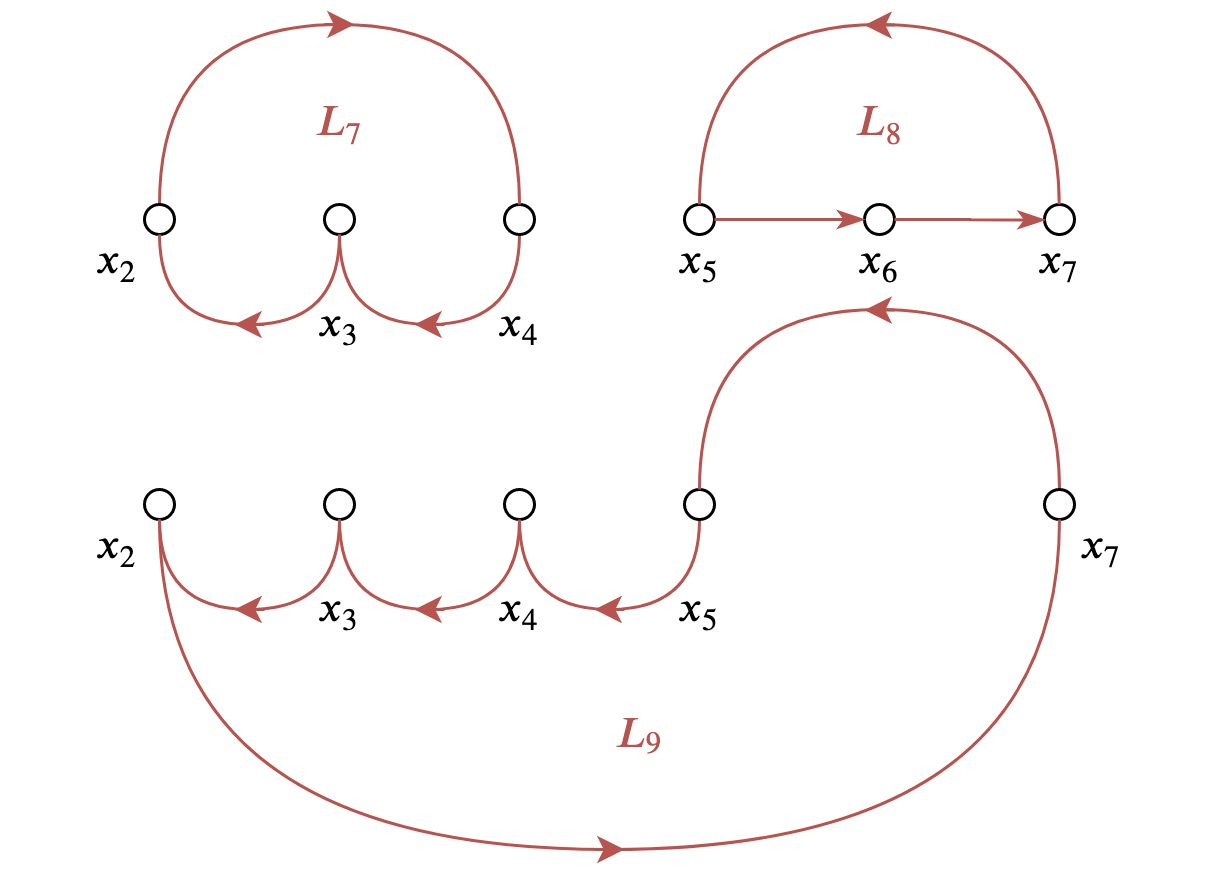
\includegraphics{lec3/Feedbacks - 2} 
		\end{marginfigure}
		\begin{figure}[h]
			\raggedleft
			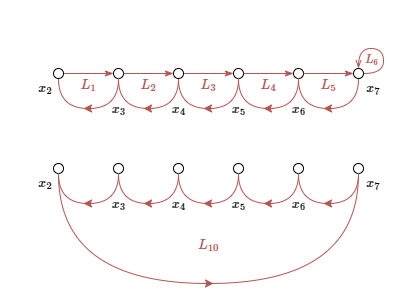
\includegraphics[width=\marginratio\textwidth]{lec3/Feedbacks - 1}
		\end{figure}
	
	\item[Self loop]  A feedback loop consisting of a single branch.
		\begin{figure}[h]
			\raggedleft
			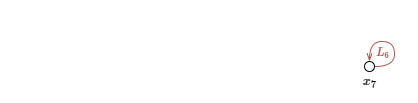
\includegraphics[width=\marginratio\textwidth]{lec3/A loop}
		\end{figure}
		
\end{description}

\subsection{Non-touching loops}

\begin{description}
	\item[Source Nodes]  Represent independent variables and have only outgoing branches. ($x_1$)
	\item[Sink Nodes]  Represent dependent variables and have only incoming branches. ($x_8$)
	\item[Mixed Nodes]  Have both incoming and outgoing branches. ($x_2 \to x_7$)
\end{description}

\subsection{Gain}
	
\begin{description}
	\item[Source Nodes]  Represent independent variables and have only outgoing branches. ($x_1$)
	\item[Sink Nodes]  Represent dependent variables and have only incoming branches. ($x_8$)
	\item[Mixed Nodes]  Have both incoming and outgoing branches. ($x_2 \to x_7$)
\end{description}

\section[Block to Flow-graph]{Block Diagram to Signal Flow Graph}
\labsec{sec3.3}

\blindtext

\section[Flow-graph Algebra]{Flow-graph Algebra\linkT{Reference: Feedback control system analysis and synthesis}}
\labsec{sec3.3}

\blindtext

\section{The Mason Rule}
\labsec{sec3.4}

\blindtext

